\documentclass[12pt,twoside,a4paper]{scrartcl}

\usepackage{prakstyling}
\usepackage[paper=a4paper,left=20mm,right=20mm,top=20mm,bottom=20mm]{geometry}
\usepackage{wrapfig}
\usepackage{amsmath}
\usepackage{hyperref}

%Für Literaturverzeichnis

\usepackage{biblatex}
\addbibresource{Bibliography.bib}



%%%%%%%%%%%%%%%%%%%%%%%%%%%%%%% Autoreninfo %%%%%%%%%%%%%%%%%%%%%%%%%%%%%%%%%%%%%%%%%%%%%%%%%%
\author{Philipp Rosendahl Mat.-Nr: 378092\thanks{philipp.rosendahl@rwth-aachen.de}
		\and Lennart Wilde, Mat.-Nr: 381588\thanks{lennart.wilde@rwth-aachen.de}}

\pSetShortAuthor{378092 \& 381588}
%%%%%%%%%%%%%%%%%%%%%%%%%%%%%%%%%%%%%%%%%%%%%%%%%%%%%%%%%%%%%%%%%%%%%%%%%%%%%%%%%%%%%%%%%%%%%

%%%%%%%%%%%%%%%%%%%%%%%%%%%%%%%%%%%%%%%% TITEL %%%%%%%%%%%%%%%%%%%%%%%%%%%%%%%%%%%%%%%%%%%%%%
\pSetTitlePrefix{Versuch}
\pSetTitleNumber[PET]
\pSetLongSubject{Physikalisches Fortgeschrittenenpraktikum - Gruppe 59} \pSetShortSubject{Gruppe 59}
%%%%%%%%%%%%%%%%%%%%%%%%%%%%%%%%%%%%%%%%%%%%%%%%%%%%%%%%%%%%%%%%%%%%%%%%%%%%%%%%%%%%%%%%%%%%%

\setlength{\parindent}{0pt}
\pagenumbering{roman}

\raggedbottom

\renewcommand{\tablename}{Tab.}
\renewcommand{\figurename}{Fig.}
\setlength{\abovecaptionskip}{1ex}
\setlength{\belowcaptionskip}{1ex}
\setlength{\floatsep}{1ex}
\setlength{\textfloatsep}{1ex}

\begin{document}

\maketitle
\newpage

\tableofcontents
\newpage

\pagenumbering{arabic}

\section{Einleitung}

	Die PET ist ein wichtiges Bildgebendes Verfahren in der modernen Medizin um auch kleine Tumore im menschlichen Körper ausfindig zu machen. Daher ist die Entwicklung leistungsfähiger Detektoren ein wichtiger Aspekt moderner Forschung. \\

	Das zugrunde liegende Prinzip basiert auf der besonders hohen Biologischen Aktivität von Tumorgewebe. Wir einem Patienten nun ein mit einem Radioaktiven Isotop markierter Zucker (sog. Tracer) verabreicht, sammelt sich dieser in dem Tumor an. Wenn dieser nun zerfällt emittiert er Positronen die sich mit den Elektronen im umliegenden Gewebe auslöchen und zwei Gamma Photonen in entgegengestezte Richtung aussenden. Diese sollen durch die Detektoren aufgefangen und ausgewertet werden um Informationen über Flugzeit und Energie der Strahlung zu erhalten. Für die Konstruktion dieser Detektoren gibt es mehrere Ansätze, allerdings wurde in diesem Experiment ein Silicon-Photomultiplier (SiPM) zusammen mit einem LYSO Szintillator verwendet.\\

	Ein auftreffendes Gamma-Photon regt den Szintillierenden Kristall nun an optische Photonen auszusenden, die auf den SiPM treffen. Dort werden sie in ein elektrisches Signal umgewandelt, welches durch einen ASIC ausgelesen und verarbeitet werden kann, um aus der Anzahl der Photonen die Energie des detektierten Photons sowie die Flugzeit udn Position zu rekonstruieren. In einem medizinischen PET-Scanner kann mit diesen Informationen nun die Lage der Tumoren im Patienten errechnet werden. In diesem Versuch ist allerdings eher die Vermessung des verwendeten Detektors im Fokus, weswegen nur zwei sich gegenüberstehende Detektoren verwendet werden.

	\newpage

\section{Versuchsaufbau}

	Der Aufbau besteht aus verschiedenen Teilen:
	\begin{itemize}
		\item Dunkelbox mit
		\begin{itemize}
			\item 2 $\gamma$-Detektoren
			\item Backbone
			\item Aluminiumgstell mit Schrittmotoren für Probenhalter
			\item Probenhalter für Radioaktive Probe
			\item
		\end{itemize}
		\item Netzteile für Detektoren und Backbone
		\item Data Aquisition and Processing Server (DAPS)
		\item Kühlung
		\item Steuerungsrechner mit Benutzerinterfaces
	\end{itemize}

	\begin{figure}[H]
		\centering
		\includegraphics[width = 0.7\textwidth]{Pictures/Netzteile.jpg}
		\label{Aufbau::Netzteile}
		\caption{Netzteile mit verschiedenen Spannungen}

	\end{figure}

	\begin{figure}[H]
		\begin{minipage}{0.69\textwidth}

					\includegraphics[width = 0.8\textwidth]{Pictures/Kammer.jpg}
					\label{Aufbau::Kammer}
					\caption{Geöffnete Dunkelkammer}

		\end{minipage}
		\begin{minipage}{0.3\textwidth}

					\includegraphics[width = 0.8\textwidth]{Pictures/Kühlung.jpg}
					\label{Aufbau::Kühlung}
					\caption{Wasserkühlung}
		\end{minipage}
	\end{figure}


	Um den Aufbau einzuschalten, muss zuerst die Kühlung gestartet werden. Danach werden die LOW, MID und HIGH Spannungen des Backbone in dieser Reihenfolge eingeschaltet. Daraufhin bootet dieser, wobei der vollständige Start durch einen Sprung in der Stromaufnahme der HIGH-Versorgungsspannung festgestellt werden kann. Nachdem der Backbone gestartet ist, können die 2 Detektoren (SPUs) eingeschaltet werden, indem wie schon bei dem Backbone zuerst die Versorgungsspannungen in der Oben angegebenen Reihenfolge sowie die BIAS-Spannung eingeschaltet werden. Auch hier ist die Betriebsbereitschaft durch einen Sprung in der Stromaufnahme auf ungefär 1.6 A erkennbar. Nun kann der Steuerungsrechner mit dem Aufbau verbunden werden. Dazu startet man die \glqq Hyperion\grqq \ Software und führt dort das zu dem Versuch gehörenden Startskript aus. Daraufhin wird eine Verbindung hergestellt, die Detektoren initialisiert und mit dem Backbone synchronisiert. Aufgrund von sporadisch auftretenden Verbindungsproblemen zwischen Backbone und den SPUs kann dieser Schritt fehlschlagen, worauf dann die Spannungen un der umgekehrten Reihenfolge abgeschaltet und der Aufbau neu gestartet werden muss.
	Ist erfolgreich eine Verbindung zwischen allen Komponenten hergestellt, sollte spätenstens nun die Dunkelkammer geschlossen werden, da im nächsten Schritt die Bias-Spannungen an die SiPMs angeschlossen werden. Wären diese nun nicht im dunklen würden sie konstant ausgelöst, was Messungen unmöglich macht und sie außerdem beschädigen kann. Ist die Kammer also geschlossen, kann mit dem Skript \glqq Continue\_Start \grqq der Aufbau in einen Messbereiten Zustand versetzt werden.

	\section{Kalibration des Probenhalters}

		\subsection{Ziel}
			Da die Steuerungssoftware mit eigenen Einheiten (nachfolgend \glqq Pulse\grqq genannt) arbeitet, muss zuerst ermittelt werden wie sich diese zu dem tatsächlich verfahrernen Strecken des Probenhalters verhalten.

		\subsection{Aufbau und Durchführung}
			Am unteren Ende des Schlittens, auf dem sich der Probenhalter befindet, ist eine Ablesenadel für einen Metermaßstab angebracht. Der entsprechende Maßstab ist unter dieser aud dem Aluminiumprofil des Aufbaus angebracht. Zum Start der Messung wird der Motor mittels der Kontrollsoftware in seine Startposition gebracht, bei der er 0 Pulse verfahren ist. Dann lässt man diesen 5000 Pulse vorfahren und liest die Aktuelle Position des Schlitten auf dem Maßstab ab. Dies wird so lange wiederholt, bis der Schlitten am Endstop Schalter auf der anderen Seite angekommen ist.

		\subsection{Auswertung}

			Es wurden bei der Messung folgende Daten aufgenommen:

				\begin{table}[H]
    \centering
    \caption{Rohdaten Kalibration}

    \begin{tabular}{| c | c |}
      Pulse & Strecke in $\si{\per \centi \metre}$ \\
                              \hline
                              $ 0 $ & $0$
    \end{tabular}
\end{table}



			Es ist sinnvoll anzunehmen dass die verfahrene Strecke und die ausgegebenen Pulse in einem linearen Zusammenhang stehen, daher wird die Modellfunktion
			\begin{align*}
					s = m \cdot x + b
			\end{align*}
			angenommen.
			Mitilfe eines Python Skriptes wird nun die Funktion an die aufgenommenen Messdaten gefittet:

			\begin{figure}[H]
				\centering
					\includegraphics[width=\textwidth]{Plots/WegKalib.png}
				\caption{Gradenanpassung an gemessene Daten}
			\end{figure}

				Damit folgt ein Umrechnungsfaktor von $m = \qty(-0.0004234 \pm \mathcal{O}(10^{-13})) \frac{\si{\centi \metre}}{\text{Puls}}$ bei einem Offset von $b = (\SI{35.370}{\centi \metre} \pm \SI{0.0003}{\centi \metre})$.


	\section{Dark Count Map}
	\label{DCM}

		\subsection{Aufbau und Durchführung}

			Aufgrund des thermischen Rauschens der Dioden, sowie Herstellungsprzessen und -ungenauigkeiten haben diese eine sog. \glqq Dunkelzählrate\grqq, d.h. eine Signalausgabe bei nicht vorhandener Stimulation. Um nun einzelne Dioden mit besonders hoher Rate zu erkennen und abzuschalten, wird vor der ersten Messung eine \glqq Dark Count Map\grqq der SiPMs ohne eine Probe erstellt. Mithilfe dieser kann man nun ermitteln welche SPADs abgeschaltet werden sollten, um eine Reduzierung der Dunkelzählrate ohne eine zu hohe Reduktion der anderen Genauigkeiten zu errreichen.\\
			Zur Durchführung der Messung wird der Aufbau wie oben beschrieben eingeschaltet und das Skript zum Aufnehmen der Messung gestartet. Dies dauert einige Minuten, und nach Abschluss werden die Daten auf dem DPAS gespeichert und müssen von dort auf den Rechner übertragen werden.

		\subsection{Auswertung}

			Die aus der Messung erhaltenen Daten lagen als eine Datei mit Tab seperierten Werten (TSV) vor (siehe Rochdatenverzeichnis). Um eine einfache Übersicht über die Sensoren zu erhalten wurde die Datei nun meit einem Python Skript eingelesen und die enhalten Zählraten in einer 2D-Grafik angezeigt:

			\begin{figure}[H]
				\begin{minipage}{0.49 \textwidth}
					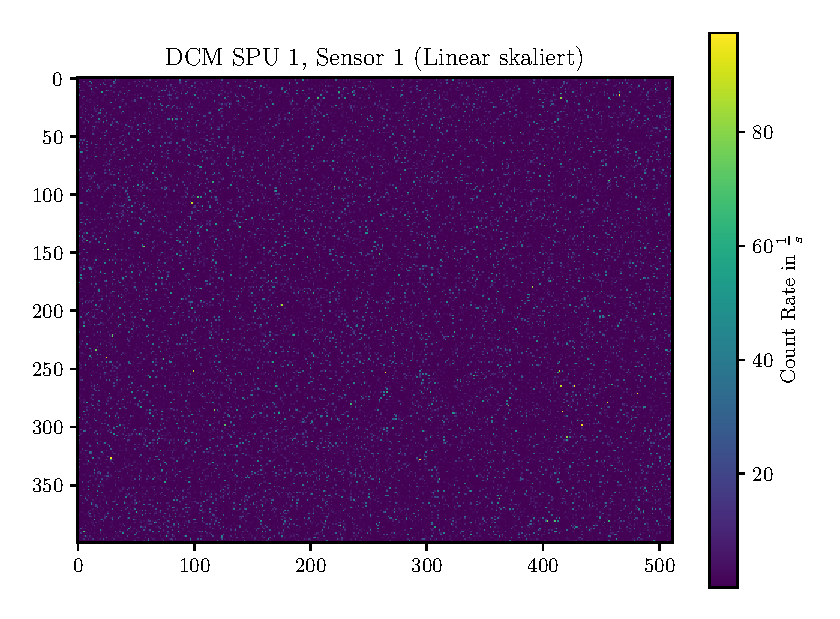
\includegraphics[width = \textwidth]{Plots/DCM/DCM_SPU1_Sensor1_lin.eps}
					\caption{Dark Count Map von SPU 1, Sensor 1}
				\end{minipage}
				\begin{minipage}{0.49 \textwidth}
					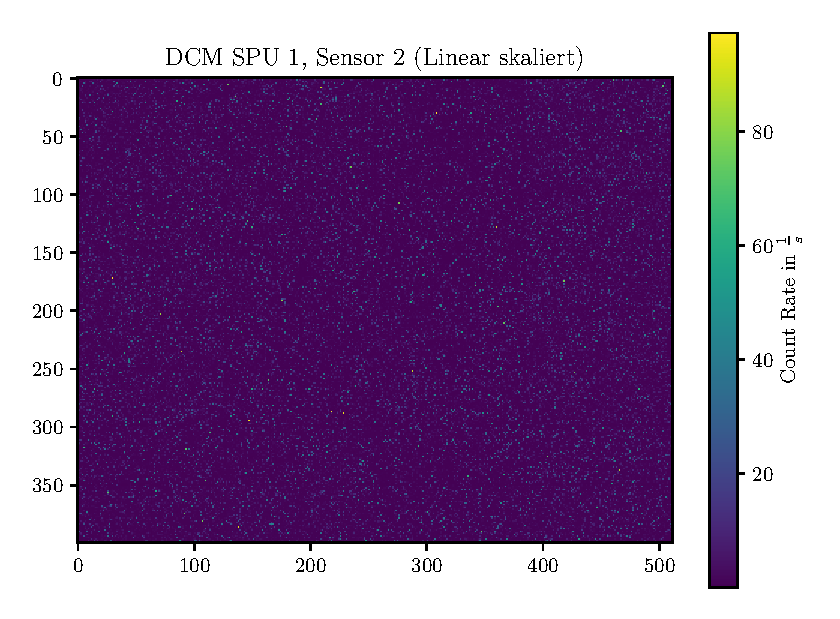
\includegraphics[width = \textwidth]{Plots/DCM/DCM_SPU1_Sensor2_lin.eps}
					\caption{Dark Count Map von SPU 1, Sensor 2}
				\end{minipage}
			\end{figure}

			\begin{figure}[H]
				\begin{minipage}{0.49 \textwidth}
					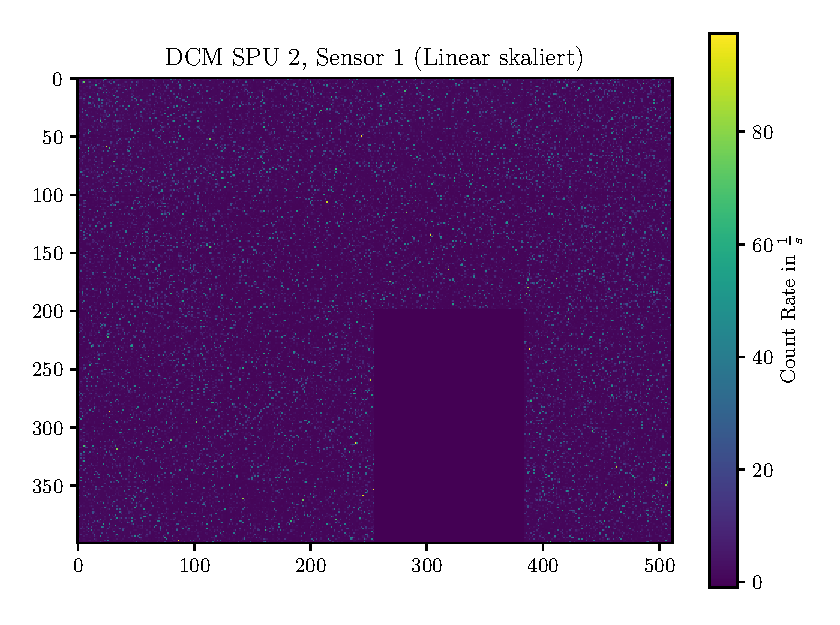
\includegraphics[width = \textwidth]{Plots/DCM/DCM_SPU2_Sensor1_lin.eps}
					\caption{Dark Count Map von SPU 2, Sensor 1}
				\end{minipage}
				\begin{minipage}{0.49 \textwidth}
					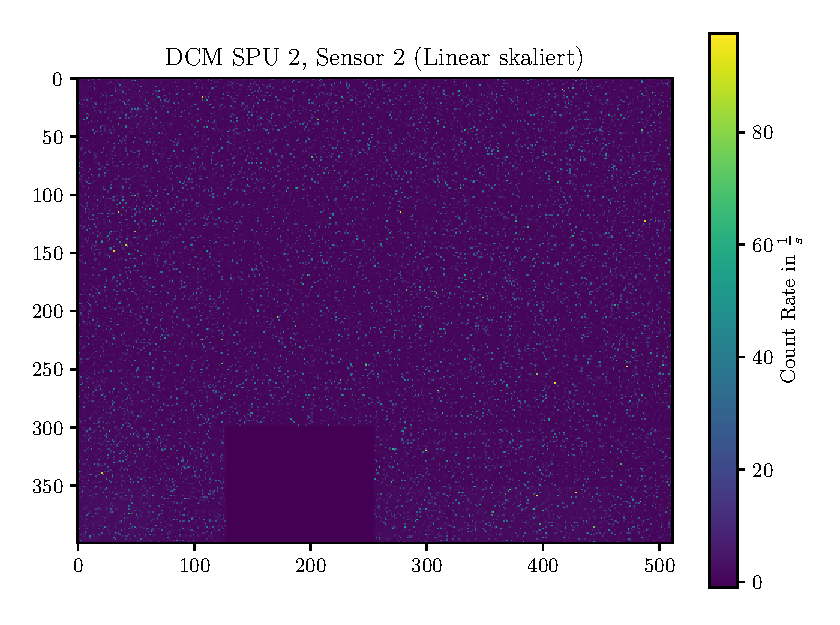
\includegraphics[width = \textwidth]{Plots/DCM/DCM_SPU2_Sensor2_lin.eps}
					\caption{Dark Count Map von SPU 2, Sensor 2}
				\end{minipage}
			\end{figure}
			Man kann erkennen dass die SPADs der Sensoren im allgemeinen geringe Dark Count Rates aufweisen, wobei einige wenige, den großteil der gesamten Rate ausmachen.
			In den Messdaten von SPU 2 ist auffällig, dass Cluster von SPADs ausgefallen sind, was auch in den Rohdaten der Messung so vorzufinden ist, sodass ein Auswertungsfehler unwahrscheinlich ist.
			Außerdem wird auf den Anhang \ref{Anhang} verwiesen in dem die Plots noch einmal größer und linear sowie logarithmisch skaliert zu finden sind.

			Außerdem wurde die Gesamtzählrate in Abhängigkeit von den abgeschalteten SPADs, wobei SPADs mit höherer Zählrate früher abgeschaltet wurden, ermittelt:

			\begin{figure}[H]
				\centering
				\includegraphics[width = 0.9 \textwidth]{Plots/DCM/DCR_vs_N.png}
				\caption{Dunkelzählrate der SPUs}
			\end{figure}

		\subsection{Fazit}

		Man sieht das N SPADs für einen Großteil des Rauschens sorgen, der durch die Abschaltung dieser eliminiert werden kann. Für die weiteren Messungen ist dies leider nicht sonderlich relevant, da für die Sensoren vorkonfigurierte Prarameter verwendet wurden, in die wir leider keine Einsicht hatten.

	\section{Rauschmessung}

	\subsection{Ziel}

		Da sowohl das im Szintillator enthaltene Lutetium selbst radioaktiv ist, als auch die Umgebung eine natürliche Strahlenbelastung aufweist, ist es nötig vor der ersten Messung eine Rauschmessung vorzunehmen um die statistischen Messfehler des Detektors abschätzen zu können.

	\subsection{Aufbau und Durchführung}

		Der Aufbau wird wie schon im Abschnitt \ref{DCM} ohne das radioaktive Präparat hochgefahren, und es wird gewartet bis sich die Temperatur der SPUs stabilisiert hat.
		Dann wird mit dem Skript \glqq Start Scan\grqq die Messung gestartet und die Ansicht in der Hyperion-Software auf das Energie Histogramm gewechselt. Dort sind dann die Histogramme für einzeln auftreffende Photonen (Singles) und Koinzident auftreffende Photonen (Coincidences) sichtbar. Nach einigen Minuten kann die Messung mit \glqq Stop Scan\grqq beendet werden, und beide Histogramme werden gespeichert.

		\subsection{Auswertung}

		Die in der gespeicherten Datei enthaltenen Daten werden durch ein Python Porgramm aufbereitet und ausgewertet.
		Es folgen Plots für die Energie-Histogramme von Singles und Koinzidenzen.

		\begin{figure}[H]
				\begin{minipage}{0.49 \textwidth}
					\includegraphics[width=\textwidth]{Pictures/Platzhalter.jpg}
					\caption{Histogramm Singles}
				\end{minipage}
				\begin{minipage}{0.49 \textwidth}
					\includegraphics[width=\textwidth]{Pictures/Platzhalter.jpg}
						\caption{Histogramm Koinzidenzen}
					\end{minipage}
		\end{figure}

		Man kann hier deutlich sehen dass kaum Koinzidenzen gemessen werden, was darauf schließen lässt dass die Photonen nicht aus einem Ereignis stammen.
		Außerdem kann mit diesen Messungen das Hintergrundrauschen der Singles gut eliminiert werden.

		\subsection{Fazit}

		\textbf{TODO}

	\section{Detektorsensitivität und Count Rate}

		\subsection{Aufbau und Durchführung}

			Das radioaktive Na-22 Präparat wird in den Probenhalter eingesetzt, und die minimalen Abstände der Probe zu dem beiden Sensoren vermessen. Nun wird die Dunkelbox geschlossen und der Aufbau wie schon in den beiden vorherigen Abschnitten eingeschaltet. Nachdem sich wieder eine stabile Temperatur an den Sensoren eingestellt hat, wird der Schlitten mit dem Probenhalter in die Mitte zwischen den beiden Detektoren verfahren und um diesen Punkt so mittels einer binären Suche so lange verfahren bis die Summe der Count-Rate der Detektoren maximal ist. Anschließend wurde das Messystem zurückgesetzt und die Count-Rate der Sensoren gespeichert.

		\subsection{Auswertung}

			Um die Detektorsensitivität zu bestimmen, kann man die theoretische Aktivität der Probe mit der tatsächlich gemessenen vergleichen.
			Dabei ist allerdings zu beachten dass durch die begrenzte Detektorfläche nur ein gewisser Anteil der tatsächlich abgestrahlten Positronen auch gemessen werden kann.
			Unter der Annahme dass die Positronen gleichmäßig unter allen Raumwinkeln abgestreut werden, muss nun als Korrekturfaktor der Anteil des Raumwinkels der Detektorfläche an der Vollkugel berechnet werden. Dann folgt mit $d$ als Abstand der Probe vom Detektor und b als halbe Seitenlänge dieses:

			\begin{align*}
				\Omega &= \int_0^2 \pi \int_0^\vartheta \sin(\theta) \dd{\phi} \dd{\theta}\\
							 &= 4 \arctan{ \frac{b^2}{2d \sqrt{4d^2 + 2b^2}}} \\
				\\
				\frac{2 \cdot \Omega_{\text{Detektor}}}{\Omega_{\text{Kugel}}} &=  \frac{8 \cdot \arctan{\qty(\frac{a\cdot b}{2d\sqrt{4d^2 + a^2 + b^2}})}}{4 \pi}
			\end{align*}

			Im Versuch wurden dabei $a$, $b$ und $d$ zu

			\begin{align*}
					a &= \SI{32.6}{\milli \metre} \pm \SI{0.1}{\milli \metre} \\
					d &= \SI{65.7}{\milli \metre} \pm \SI{0.1}{\milli \metre}\\
					b &= \SI{26}{\centi \metre}\pm \SI{1}{\centi \metre}
			\end{align*}

			vermessen. Damit ergibt sich für die Geometrische Effizienz:

			\begin{align*}
				G &= 0.005 = 0.5 \%
			\end{align*}

			Außer der geometrischen Effizienz ist allerdings noch die des Szintillatormaterials, sowie der SiPM zu berücksichtigen. Wenn das Detektormaterial zu dünn ist, haben die $\gamma$-Photonen nicht genügend Strecke um ihre Energie zu verlieren. Man kann annehmen dass die Energieabgabe im Material einem exponentiellen Abfall

			\begin{align*}
				\frac{I}{I_0} =  \cdot e^{-\frac{x}{\mu}}
			\end{align*}

			mit $\mu$ als Habwertsdicke folgt. Damit kann man nun die gesamte Energieabgabe im Kristall berechnen.

			Für den hier verwendeten LYSO-Kristall ist die Halbwertsdicke $\mu = \SI{11}{\milli \metre}$

			Damit folgt mit der Dicke des Detektors von $\SI{12}{\milli \metre} \pm \SI{0.1}{\milli \metre}$:

			\begin{align*}
				\frac{I}{I_0} = e^{\frac{\SI{12}{\milli \metre}}{\SI{11}{\milli \metre}}} \approx 0.33 \%
			\end{align*}


			Da außerdem die radioaktive Probe zerfällt, verringert sich ihre Aktivität mit der Zeit. Um die Sensitivität zu berechnen, muss nun allerdings die Aktivität der Probe bekannt sein. Sie folgt auch einem Exponentiellen Abfall:

			\begin{align*}
				A = A_0 \cdot 2^{- \frac{t}{t_0}}
			\end{align*}

			mit $t_0 = 2.6 a$ als Halbwertszeit der Probe. Die im Versuch verwendete Probe hatte am 1.4.2013 eine Aktivität von $\SI{1.11}{\mega \becquerel}$. Damit ergibt sich eine Aktivität von

			\begin{align*}
				A = A_0 \cdot 2^{- \frac{6.83}{2.6}} = \SI{0.18}{\mega \becquerel}
			\end{align*}

			am Versuchstag.

			Dies kann schlussendlich mit der vom Detektor gemessenen Aktivität der Probe verglichen werden.

			Diese wird durch die Koinzidenzrate bei $\SI{511}{\kilo \electronvolt}$ beschrieben, und beläuft sich auf:

			\begin{align*}
				A_{gemessen} =
			\end{align*}

		\subsection{Fazit}



	\section{Energiemessung}

	\subsection{Aufbau und Durchführung}
		Mittels der Hyperion Steuerungssoftware wurde die Messung gestartet, und auf die Energieansicht gewechselt. Als Messdauer wurde gewartet, bis ein Peak mindestens 100 Datenpunkte erricht hatte.


	\subsection{Auswertung}

		Die Daten wurden aus der mit Hyperion exportierten CSV Datei mit einem Python Skript \footnote{\url{https://github.com/Lenni/F_Praktikum}} weiter verarbeitet. Dabei wurde das Rauschen der Sensoren wurde auf die Messzeit normiert und von den Messdaten subtrahiert. Mithilfe der bekannten Peaks bei $511 \si{\kilo \electronvolt}$ und $1275 \si{\kilo \electronvolt}$ wurde die Energieskala kalibriert. Um die Mittelpunkte und Fehler auf die Spitze der Peaks zu finden wurde eine Gaußverteilung an den jeweiligen Peak gefittet, wobei dann die Standardabweichung den Fehler auf den Messwert und der Mittelwert der Verteilung den Messwert selbst darstellt.

		Die dabei in den Fit eingehenden Fehler setzen sich aus dem Binning der Detektoren zusammen.

		Man erhält nun folgendes Diagramm mit Residuenplots für die oben erwähnten Fits:

		\begin{figure}[H]
				\centering

				\includegraphics[width = 0.5 \textwidth]{Plots/EnergyUnkorrigiert511 Peak.png}


					\caption{Unkorrigierter 511 keV Peak}
		\end{figure}

		Um die Energieskala des Detektors zu Kalibrieren kann der Mittelwert des $\SI{511}{\kilo \electronvolt}$ bestimmt werden, und durch Division des erwarteten- durch den bestimmten Wert ein Korrekturfaktor berechnet werden. Alle Energien können nun mit diesem multipliziert werden um das kalibrierte Enegiespektrum zu erhalten.
		Die Qualität dieser Korrektur kann man nun auch durch den Mittelwert des $\SI{1275}{\kilo \electronvolt}$ Peaks begutachten, da dieser nun auch möglichst nah (innerhalb der Fehler) an seinem erwarteten Wert sein sollte.


		\begin{figure}[H]
			\centering
			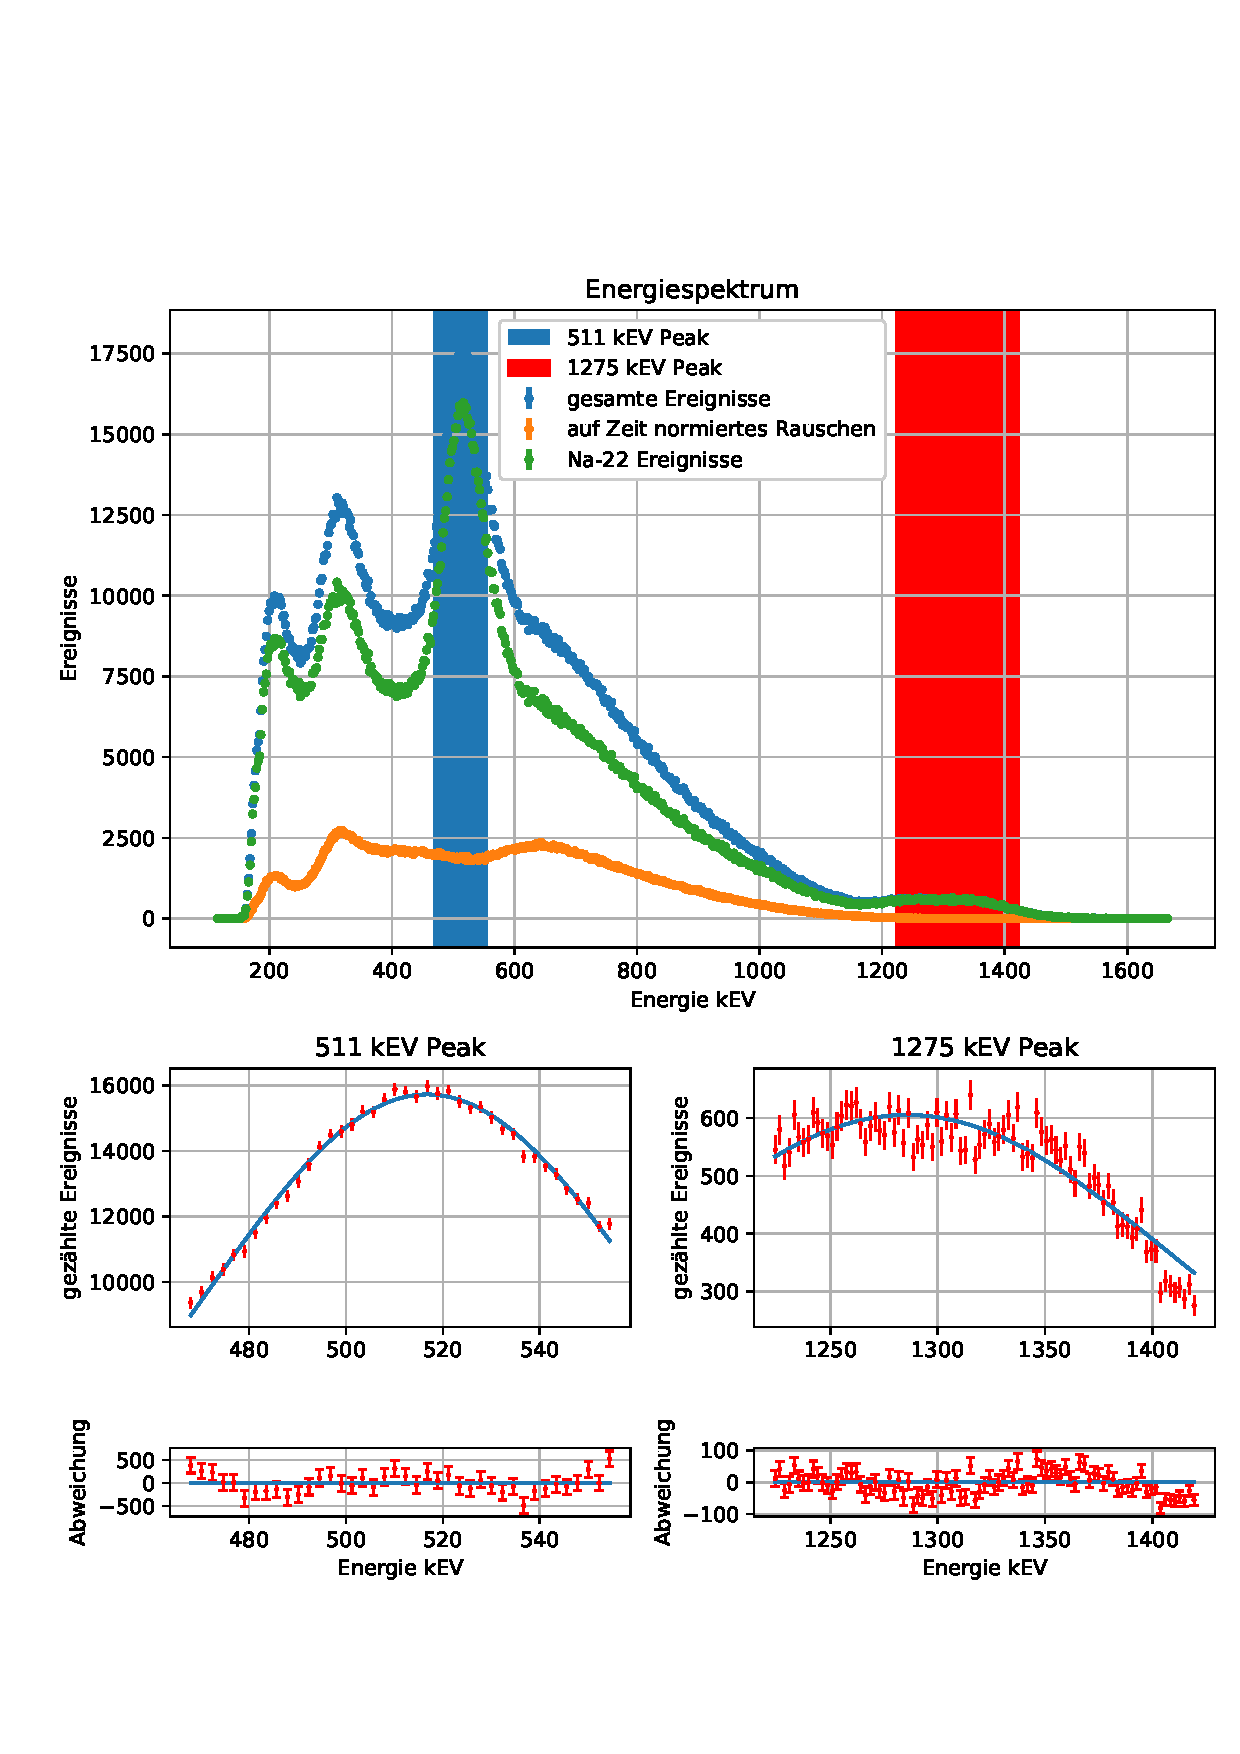
\includegraphics[width = \textwidth]{Plots/energy_resultion.png}
			\caption{Energieauswertung}
		\end{figure}

		Dabei sind die transparent markierten Bereiche die angenommenen Fehler auf die Peaks.

		Man kann erkennen dass der Mittelwert des $\SI{1275}{\kilo \electronvolt}$-Peaks sehr gut innerhalb des rötlichen Bereiches liegt, womit die Korrektur als hinreichend gut angenommen wird. Allerdings ist zu beachten, dass aufgrund der vergleichsweise geringen Dicke der Detektoren nur eine geringe Menge der tatsächlichankommenden Photonen korrekt gemessen wird. Dies resultiert in einem großen Fehler auf diesen Peak. Da nun alle Energiewerte mit einem konstanten Faktor multipliziert wurden, ergibt sich daraus ein etwas größerer Fehler auf alle Energien.

\subsection{Fazit}

		Man kann an den Messungen erkennen, dass der verwendete Detektor eine Energieauflösung von $\Delta E = \SI{000}{\kilo \electronvolt}$ besitzt. Diese könnte durch eine andere Detektor-Szintillator Koppelung noch erhöht werden, allerdings resultiert daraus eine geringere Ortsauflösung.

	\section{Timing Resolution}

		\subsection{Ziel}

		\subsection{Aufbau und Durchführung}
			Das Experiment wird wie oben schon beschrieben aufgebaut und die Probe in den Probenhalter gestellt. Nun wird dieser mit der Motorensteuerung an eine zufällige Position zwischen den SPUs gefahren und die Messung gestartet. Die Position des Motors wird außerdem aus der Steuerung abgelesen und notiert, um einen Vergleich der Vorraussage mit der tatsächlichen Position zu ermoglichen. Im 'Time Difference Spectrum' der Software kann nun in einem Histogramm die Zeitdifferenz zwischen 2 als koinzident gewerteten Photonen gezeigt werden. Da die von einem der Detektoren weiter als vom anderen entfernt sind, werden die von einem auch früher detektiert. Aus der Zeitdifferenz zwischen den Signalen kann nun ein vermuteter Ursprungspunkt zwischen den beiden SPUs berechnet werden. Diese Prozedur wird nun 3 weitere Male wiederholt, wobei die Probe jedes Mal an eine andere, zufällige Position verschoben wird.

			\subsection{Auswertung}
				Um den Fehler auf die Zeitauflösung des Messystems zu erhalten, kann an das erhaltene Histogramm der mittigen Messung eine Gaußverteilung gefittet werden.

				\begin{figure}[H]
					\centering

						\includegraphics[width=\textwidth]{Plots/Time/TDS_Cal.png}

					\caption{Fit Zeitauflösung}
				\end{figure}

				Man sieht hier eine deutliche Systematik in den Residuen, die dadurch behoben werden kann, dass man sich bei den Fits auf einen bereich um die Peaks beschränkt und weit außen liegende Bereiche ignoriert.

				Damit folgt dann der Fit der modifizierten Daten:

				\begin{figure}[H]
					\centering
						\includegraphics{Plots/Time/SelTDS_Cal.png}
					\caption{Fit der angepassten Daten}
				\end{figure}

				Wie man sehen kann ist die Systematik verschwunden und die angepasst Gerade ist auch visuell näher an dem Verlauf der Daten.

				Für die Gaußverteilung
				\begin{align*}
					f(t) &= \sqrt{\frac{1}{2 \pi}} e^{-\frac{(x-\mu)^2}{2 \sigma^2}}
				\end{align*}

				werden folgende Parameter bestimmt:

				\begin{align*}
					\mu &= \SI{000}{\second} \pm \SI{000}{\second} \\
					\sigma &= \SI{000}{\second} \pm \SI{000}{\second} \\
					\frac{\chi^2}{NDF} &= ???
				\end{align*}

				An dem nicht verschwindenden Mittelwert, kann man erkennen, dass die Probe wahrscheinlich nicht perfekt mittig zwischen den Detektoren war.
				Die Standardabweichung von $\sigma = ???$ beschreibt die Koinzidenzzeit des Systems. Theoretisch sollte diese Genauigkeit ausreichen um Strecken von $\SI{000}{\centi \metre}$ aufzulösen.
				 \\
				 \\

				 Nun kann mit diesen gewonnenen Informationen die Position der Probe bei den verschiedenen Messungen ermittelt werden:

				 \begin{figure}[H]
				 		\centering

							\includegraphics[width=\textwidth]{Plots/Time/TDS_1.png}

						\caption{Zeitdifferenzen}
				 \end{figure}

				 Auch hier müssen wie oben schon beschrieben auftretende Systematiken duch die Beschränkung des Datenbereiches entfernt werden.

				 Dabei wurden folgende Daten ermittelt:

				 \begin{table}[H]
  \caption{title}

  \begin{tabular}[|c|c|c|c|]
    & Messung 1 & Messung 2 & Messung 3 \\
    \hline
    $\mu$ & 000 & 000 & 000 \\
    $\sigma$ & 000 & 000 & 000 \\
  \end{tabular}

\end{table}


				 Diese Daten lassen auf folgende Positionen der Probe schließen:

				 \begin{align*}
				 	\text{Messung 1:}& \SI{000}{\centi \metre} \pm \SI{000}{\centi \metre} \\
					\text{Messung 2:}& \SI{000}{\centi \metre} \pm \SI{000}{\centi \metre} \\
					\text{Messung 3:}& \SI{000}{\centi \metre} \pm \SI{000}{\centi \metre} \\
				 \end{align*}

				 Wenn man diese mit den tatsächlichen Positionen vergleicht, sieht man \textbf{dass wir absolut daneben lagen!}


	\newpage


	\section{}


	\section{Anhang}
		\label{Anhang}

		\subsection{Dark Count Maps}

		\begin{figure}[H]
			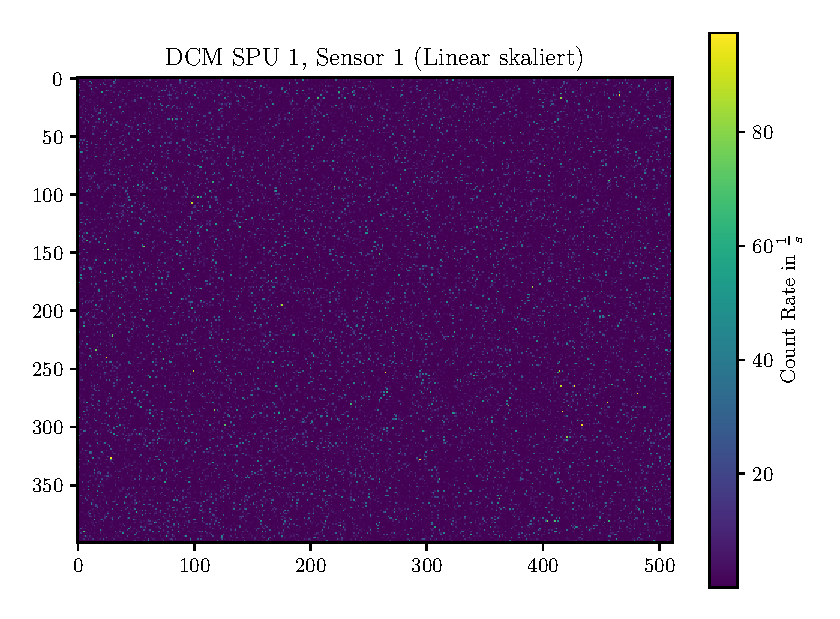
\includegraphics[width = \textwidth]{Plots/DCM/DCM_SPU1_Sensor1_lin.eps}
			\caption{DCM SPU 1, Sensor 1, Linear}
		\end{figure}

		\begin{figure}[H]
			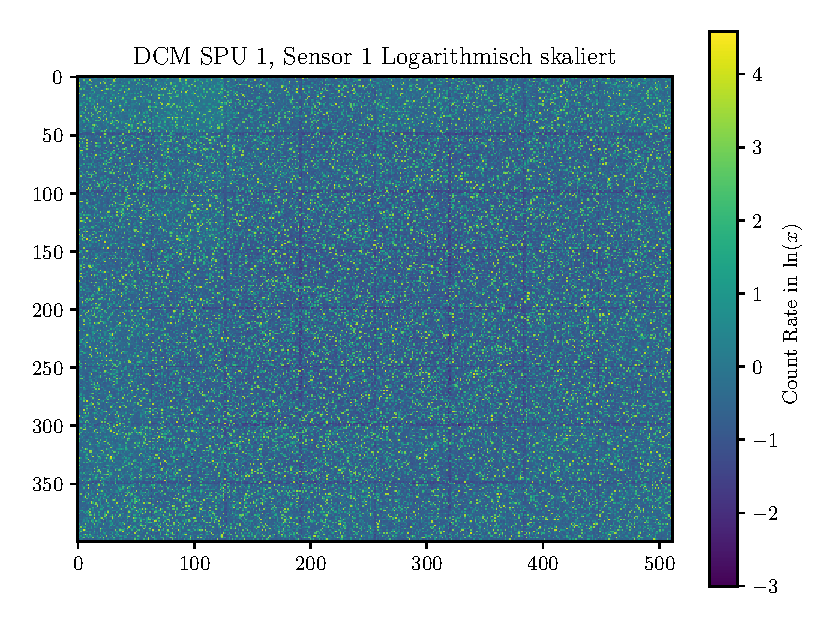
\includegraphics[width = \textwidth]{Plots/DCM/DCM_SPU1_Sensor1_log.eps}
			\caption{DCM SPU 1, Sensor 1, Logarithmisch}
		\end{figure}

		\begin{figure}[H]
			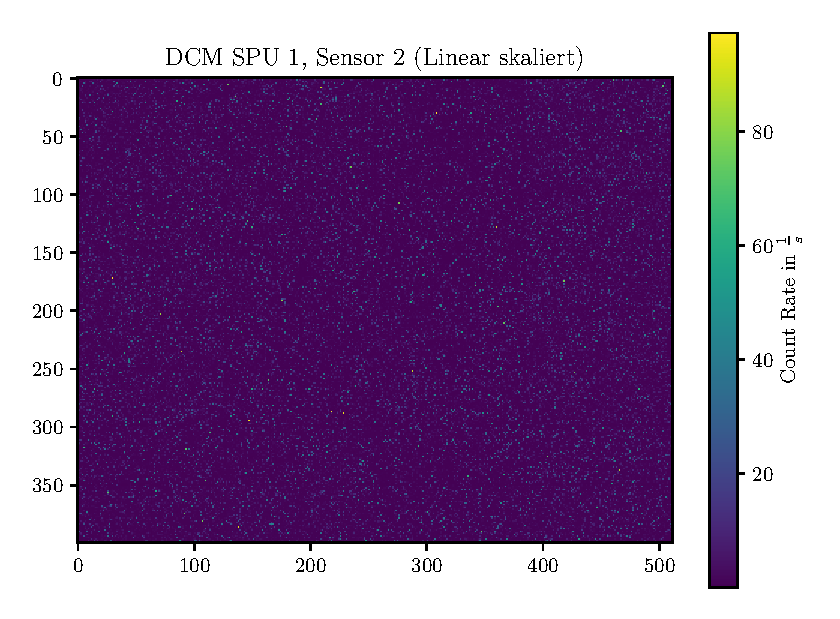
\includegraphics[width = \textwidth]{Plots/DCM/DCM_SPU1_Sensor2_lin.eps}
			\caption{DCM SPU 1, Sensor 2, Linear}
		\end{figure}

		\begin{figure}[H]
			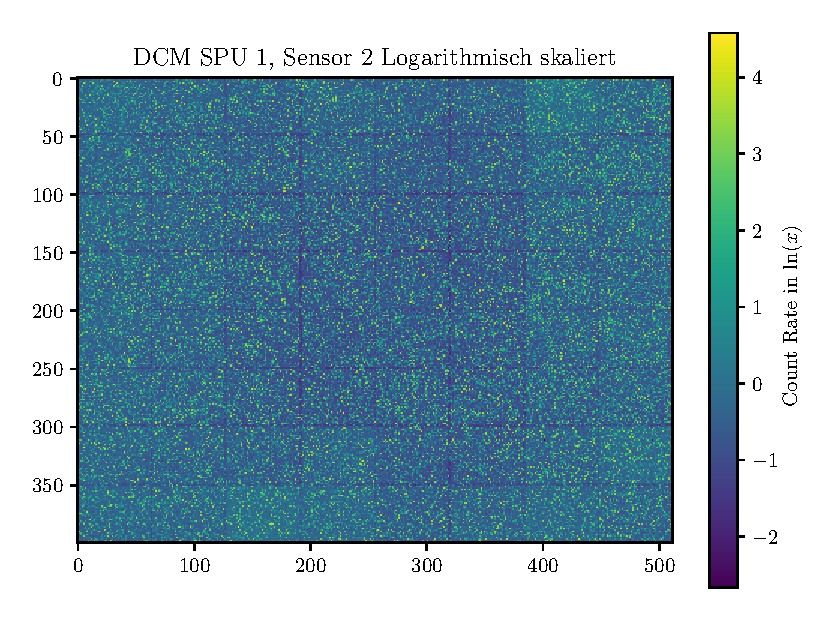
\includegraphics[width = \textwidth]{Plots/DCM/DCM_SPU1_Sensor2_log.eps}
			\caption{DCM SPU 1, Sensor 2, Logarithmisch}
		\end{figure}

		\begin{figure}[H]
			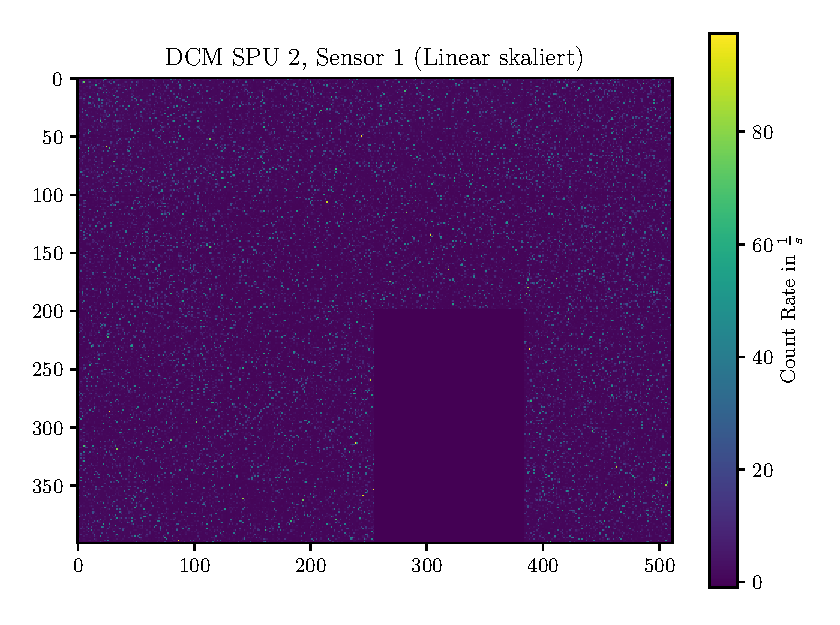
\includegraphics[width = \textwidth]{Plots/DCM/DCM_SPU2_Sensor1_lin.eps}
			\caption{DCM SPU 2, Sensor 1, Linear}
		\end{figure}

		\begin{figure}[H]
			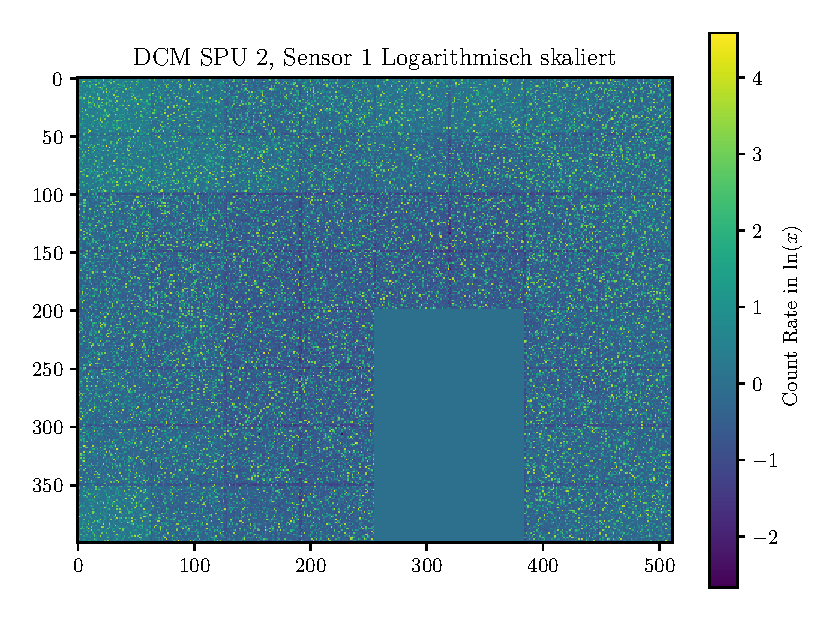
\includegraphics[width = \textwidth]{Plots/DCM/DCM_SPU2_Sensor1_log.eps}
			\caption{DCM SPU 2, Sensor 1, Logarithmisch}
		\end{figure}

		\begin{figure}[H]
			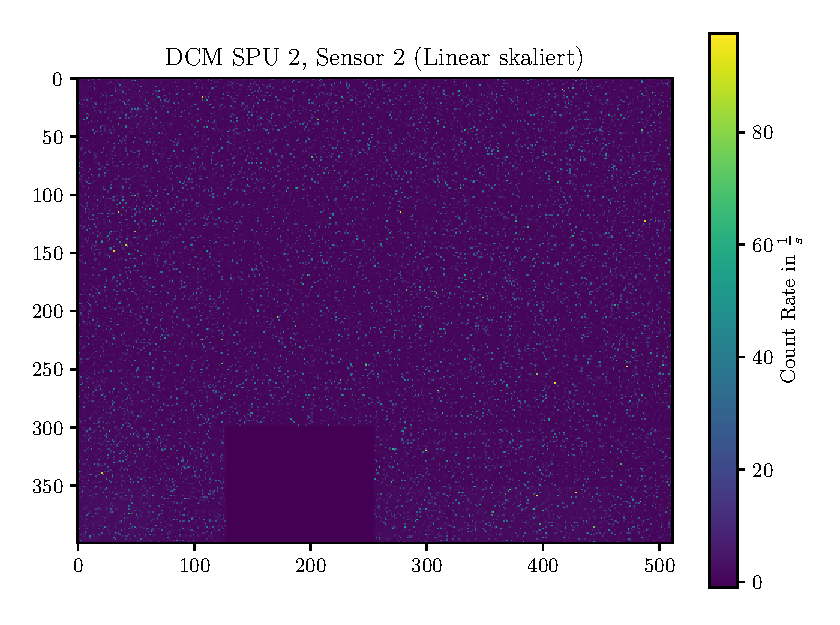
\includegraphics[width = \textwidth]{Plots/DCM/DCM_SPU2_Sensor2_lin.eps}
			\caption{DCM SPU 2, Sensor 2, Linear}
		\end{figure}

		\begin{figure}[H]
			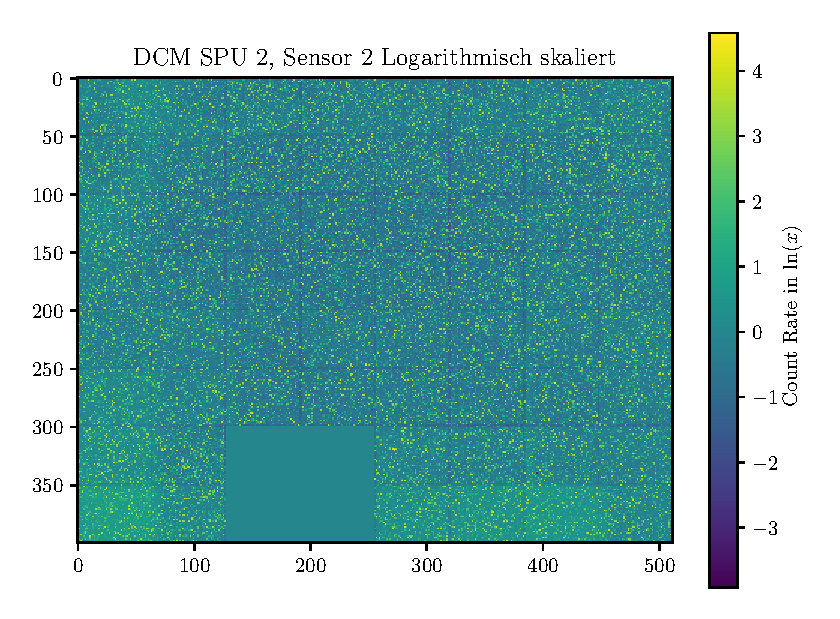
\includegraphics[width = \textwidth]{Plots/DCM/DCM_SPU2_Sensor2_log.eps}
			\caption{DCM SPU 2, Sensor 2, Logarithmisch}
		\end{figure}

\end{document}
